\documentclass[12pt, a4paper]{article}
\usepackage{caption}
\usepackage{graphicx}
\usepackage{hyperref}
\hypersetup{
    colorlinks,
    citecolor=black,
    filecolor=black,
    linkcolor=black,
    urlcolor=black
}
\usepackage{tikz-network}
\usepackage{amsmath, amsfonts, amssymb, amsthm}
\usepackage{algpseudocode}
\usepackage{algorithm}
\title{Computer Architecture\\and system programming}
\date{2022}
\author{Kristoffer Klokker}

\usepackage{xcolor,listings}
\usepackage{textcomp}
\usepackage{color}
\usepackage{listings}
\definecolor{codegreen}{rgb}{0,0.6,0}
\definecolor{codegray}{rgb}{0.5,0.5,0.5}
\definecolor{codepurple}{HTML}{C42043}
\definecolor{backcolour}{HTML}{F2F2F2}
\definecolor{bookColor}{cmyk}{0,0,0,0.90}  
\color{bookColor}

\lstset{upquote=true}

\lstdefinestyle{mystyle}{
    backgroundcolor=\color{backcolour},   
    commentstyle=\color{codegreen},
    keywordstyle=\color{codepurple},
    numberstyle=\numberstyle,
    stringstyle=\color{codepurple},
    basicstyle=\footnotesize\ttfamily,
    breakatwhitespace=false,
    breaklines=true,
    captionpos=b,
    keepspaces=true,
    numbers=left,
    numbersep=10pt,
    showspaces=false,
    showstringspaces=false,
    showtabs=false,
    tabsize=3,
}
\lstset{style=mystyle}
\usepackage{zref-base}

\makeatletter
\newcounter{mylstlisting}
\newcounter{mylstlines}
\lst@AddToHook{PreSet}{%
  \stepcounter{mylstlisting}%
  \ifnum\mylstlines=1\relax
    \lstset{numbers=none}
  \else
    \lstset{numbers=left}
  \fi
  \setcounter{mylstlines}{0}%
}
\lst@AddToHook{EveryPar}{%
  \stepcounter{mylstlines}%
}
\lst@AddToHook{ExitVars}{%
  \begingroup
    \zref@wrapper@immediate{%
      \zref@setcurrent{default}{\the\value{mylstlines}}%
      \zref@labelbyprops{mylstlines\the\value{mylstlisting}}{default}%
    }%
  \endgroup
}

% \mylstlines print number of lines inside listing caption
\newcommand*{\mylstlines}{%
  \zref@extractdefault{mylstlines\the\value{mylstlisting}}{default}{0}%
}
\makeatother


\newcommand\numberstyle[1]{%
    \footnotesize
    \color{codegray}%
    \ttfamily
    \ifnum#1<10 0\fi#1 |%
}


\begin{document}
	\maketitle
	\clearpage
	\tableofcontents
	\clearpage
	\section{The basics}
		Computer architecture: attrributes of a system visible to the programmer, such as instruction set architecture (ISA) which defines opcodes, registers, instruction and data memory.\\
		Computer organization: operational units and their interconnections, which are the behind the scenes of the architecture.\\
		\subsection{Structure and Function}
			A computer can perform 4 basic functions:
			\begin{itemize}
				\item Data processing - manipulate data in some form
				\item Data storage - in every computer some form of storage is needed even if it just temporary
				\item Data movement - data movement can be in many forms but most clear is the data movement from the input/ouput (I/O) refered to as peripheral
				\item Control - a control unit which can orchestrate the performance and functional parts of the computer
			\end{itemize}
			 This therfore creates a computer structure of:  CPU, Main memory, I/O, System bus.\\
			 The CPU are here a unit consisting of:
			 \begin{itemize}
			 	\item Control unit - Control the operations sent to the CPU
			 	\item Arithmetic and logic unit (ALU) - perform the data processing
			 	\item Registers - storage for the CPU
			 	\item CPU interconnection - communication between the different units in the CPU
			\end{itemize}
			Some processors have multiple levels of cache where the higher level the faster yet smaller cache.\\
			Some CPU may also have multiple cores which consist of: 
			\begin{itemize}
				\item ISU (instruction sequence unit) - controls instructions sequence and allows for an out-of-order (OOO) sequence
				\item IFB (instruction fetch and branch) and ICM (instruction cache and merge) - These two subunits contain the 128-kB instruction cache, branch prediction logic, instruction fetching controls, and buffers.
				\item IDU (instruction decode unit) - fed from the IFU buffer it parses and decodes architecture operation codes
				\item LSU (load-streo unit) - contains L1 data cache and controls data flow between L1 and L2 cache
				\item XU (translatio unit) - Translate logical addresses into physical addresses
				\item PC (core pervasive unit) - Collects instrument data and errors
				\item FXU (fixed-point unit) - executes fixed point arithmetic operaitons
				\item VFU (vector and floating-point unit) - Handles all binary and hexadecimal floating point operations and fixed-point multiplication
				\item RU (recovery unit) - Keep a copy of the complete state in case of recovery
				\item COP (dedicated co-processor) - data compression and encryption functions for each core
				\item L2D - data cache for memory traffic
				\item L2I - instruction cache
			\end{itemize}
		\subsection{Gates, memory cells, Chips, and Multichip modules}
			The only two required components for a digital computer are: gates and memory cells\\
			A gate is a component which implments a boolean or logical function, ex AND gate.\\
			A memory cell can be in two states at all time on or off and in this way save a bit.\\
			A transistor is the electric based implmentation of a gate or memory cell\\
		\subsection{Processor architecture}
			The Intel x86 by the complex instruction set computers (CISCs).\\
			Unlike ARM which is based on reduced instruction set computer (RISC).\\
		\subsection{Embedded systems}
			These are system which are general purpose, but system where hardware and software (embedded system (OS)) are coupled together.\\
			Theses system is found everywhere, and often working with the external envirement via sensors.\\
			Due to the software only having one purpose they are more efficient in both energy and processing power.\\
			An embedded system may use a general purpose chip but most use a dedicated processor with specific number of needed tasks.\\
			These dedicated chips often take form in microcontrollers which are sos called computers on a chips, small chips which have the same requirements for the 4 basic functions of a computer.\\
			Deeply embedded systems are microcontrolelrs with burnt in programs and no interactions with the user.
	\section{Performance}
		In order to achieve the processing power of today different methods are being used to keep task comming to the CPU
		\begin{itemize}
			\item Pipelining  - An execution of an instruction has multiple parts like: fetching instruction, decoding opcode, fetch operands and so on. Pipelining handles multiple executions by handling a different parts in every task.
			\item Branch prediction - By looking ahead in the instruction code, a prediction of needed instructions and buffers can be fetched beforehand.
			\item Superscalar execution - Multiple instructions are performed every processor clocl cycle.
			\item Data flow analysis - By observing which instructions depend on other instruction result, a new order of instruction are made.
			\item Speculative execution - By using branch prediction and data flow analysis, the CPU speculates on upcoming instruction and execute them.
		\end{itemize}
		To create a new and faster CPU there are three aproaches:
		\begin{itemize}
			\item Increase speed by reducing size of the chip, and therefore reducing the travel time of information
			\item Speed up cache size, to reduce to waiting time on slow data transformation
			\item Change processor oragnization and architecture to allow for better parallelism
		\end{itemize}
		But by increasing the speed and lowering the size of transistor, it creates new problem such as: Power density becomming higher and making it harder to dessipate heat, slower electron flow due to smaller connection which creates more resistance, Memory access speed which is a common constraint for CPUs.\\
		Therefore a more modern solution is multi core processor designs, such more cores with shared cache can archive more speed.\\
		Amdahls law describe hwo multicore can speedup a process as followed
		$$Speedup = \frac{1}{(1-f)+\frac{f}{N}}$$
		Where $f$ is the code which can infinitly be parallelizable and $N$ is the number of cores.\\
		But this should be taken with a grain of salt due to in a real envirement other processes are able to make use of extra cores in case of a non parallelizable task.\\
		A simple way to measure required speed is Littles Law which is 
		$$L=\lambda W$$
		Where $L$ is the aver number of unit in the system at any time, $\lambda$ is average rate of items which arrive per unit time and $W$ is a number of unit time.
		\subsection{Measuring performance}
			Clock speed are a way of measuring the speed of electric pulses in the CPU measured in Hz, The time between a clock tic is called cycle time.\\
			Average cycle per instruction (CPI) is the average number of cycles needed for every avaliable instruction. \\
			With this the process time can be calculated as
			$$T=I_C \times [p+(m\times l)]\times \tau$$
			$I_C$ is instruction count, $\tau=1/f$ where $f$ is clocl frequency,  $p$ number of processor cycles for decode and execute, $m$ number of memory references, $k$ ratio between memory cycle time and processor cycle time.\\
			Often the millins of instruction per second (MIPS) is used which can be found with:
			$$MIPS = \frac{f}{CPI\times 10^6}$$
			Which also can be found in variations with floating point operations (MFLOPS)\\
			This is a flawed measurement due to different architectures like RISC and CISC where RISC will always have an advantage due to the reduced instruction set.\\[4mm]
			A good benchmark should be:
			\begin{itemize}
				\item Written in hight level language to make portability high
				\item Is representive of a kind of programming domain
				\item Easily measured
				\item Wide distribution
			\end{itemize}
			SPEC is a standard for benchmarking which uses these terms:
			\begin{itemize}
				\item Benchmark - program written in high level and able to compile and execute on every computer which implments the compiler
				\item System under test - the tested computer system
				\item Reference machine - the reference scores from a choosen machine to compare current result to
				\item Base metric - strict guidelines for compilation in order to be able to comapre results
				\item Peak metric - Optimized settings for the given system
				\item Speed metic - The total time of execute a compiled benchmark
				\item Rate metric - the number of tasks which can be completed in a given amount of time
			\end{itemize}
	\section{Digital logic}
		\subsection{Boolean algebra}
			Boolean algebra are algebra based on only the values 1 or 0.\\
			It consist of variables and the operations AND ($\cdot$), OR (+) and NOT ($\overline{b}$) in that precedence.\\
			Another often usefull operators are XOR ($\oplus$), NAND ($\overline{b\cdot a}$) and NOR ($\overline{a+b}$)\\
			Set operation may also be performed on sets of boolean, where union is or, intersect is and. When applies the operation is performed on each bit one by one.\\
			And then the universal set will just be a set of 0's.\\
			For more info, checkout my logical proposition repo.\\
			\begin{figure}[h!]
				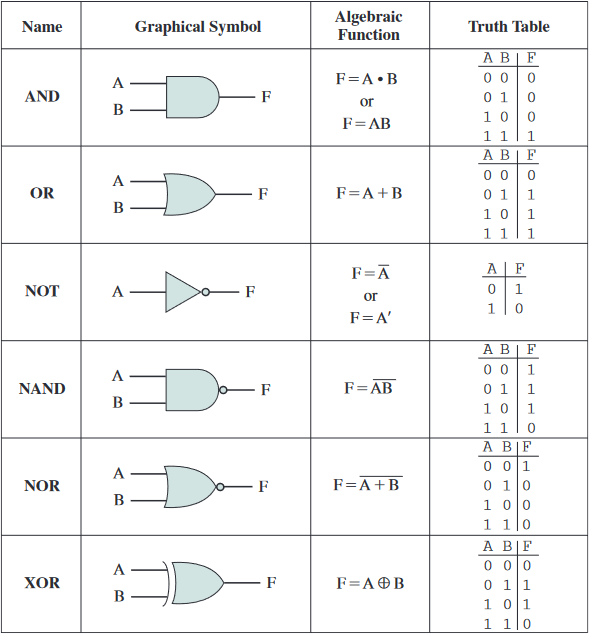
\includegraphics[width=300px]{assets/gates.png}
				\centering
				\caption{Figure of gates and their logical operation}
			\end{figure}
			These gates only have two output and one output except the NOT gate, but any number of inputs is possible and some gates may have two outputs where one is negated.\\
			When designing af circuit the fewer amount of gates the simpler and to complete possible operation the following set combinations are possible:
			\begin{itemize}
				\item AND, OR, NOT
				\item AND, NOT
				\item OR, NOT
				\item NAND
				\item NOR
			\end{itemize}
			When writing circuit, it can be done in two forms, sum of products, where product expression are multiplied, and product of sums (POS) where sum are multiplied.\\
			Both forms may not be the most simple form, but SOP uses only NAND, NOT and OR gates and POS uses only OR, AND, and NOT.\\
			To simplify a circuit there are different methods
			\begin{itemize}
				\item Algebraic simplifications - This can be done with indentities, which can simplify the expressions
				\item Karnaugh Maps - k-maps are a method which can help simplifying which variables are the out depended upon
			\end{itemize}
			
			\subsection{Karnaugh maps}
				This method works by taking 2 to 4 variables from a truthstable or function. They are then setup in a grid such all posibilities are accounted for.\\
				So for one side describing one variable there are 2 possibilites and a row which describes two variables there will be 4 possible outcomes.\\
				For each row/column combination the function or truthtable are used to determine if the cell is 0 or 1.\\
				Afterwards each 1 is circled in groups of powers of 2, so 1,2,4,8 or so on. A circle can not be cross or contain 0.\\
				For each circle the depending non changing variables are used in an and form and may be negated if the input was a consisten 0.\\
				For each circle the found AND expression is added with or to eachoter.
				\begin{figure}[h!]
					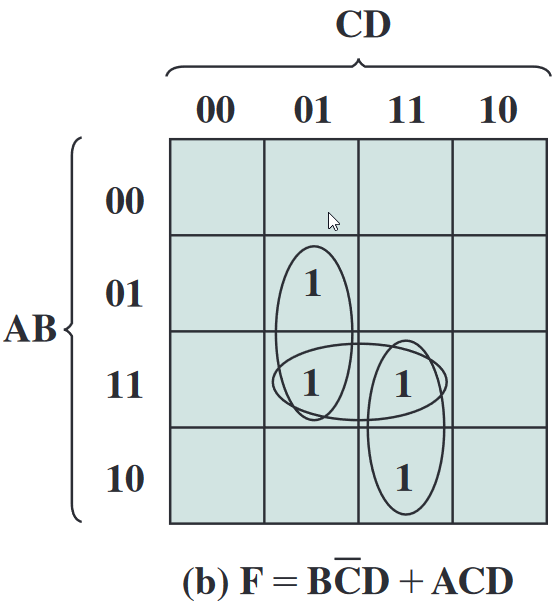
\includegraphics[width=200px]{assets/kmap.png}
					\centering
					\caption{Example of kmap and the output function}
				\end{figure}
			\subsection{Quine-McCluskey method}
				This is a more suitable method for SOP which have more than 4 variables.\\
				The method works by first creating a table with each collection of products on each row and in every column is the variables and in each cell are the needed value for the term to turn true.\\
				The table is then ordered such the row with most 0's is at the top at the row with most 1's are at the bottom.\\
				Then every row is compared to every row starting at the top, and if a row exist with only one column difference, the difference variable is eliminated and the rest of the variables are added to a new list.\\
				Then every element in the list is done with same procedure, and new found objects are added to the list. Then the same step is repeated with every new element until there is no new elements.\\
				Then every elment from the list is added to a table as rows and the original terms are added as columns.\\
				Then an X is placed in every cell where the row product is contained in the column. Then circle every X which is alone in a column, and square every X which are in a row with a circle.\\
				Those rows with a marked X are now needed for the minimal expression.
				\begin{figure}[h!]
					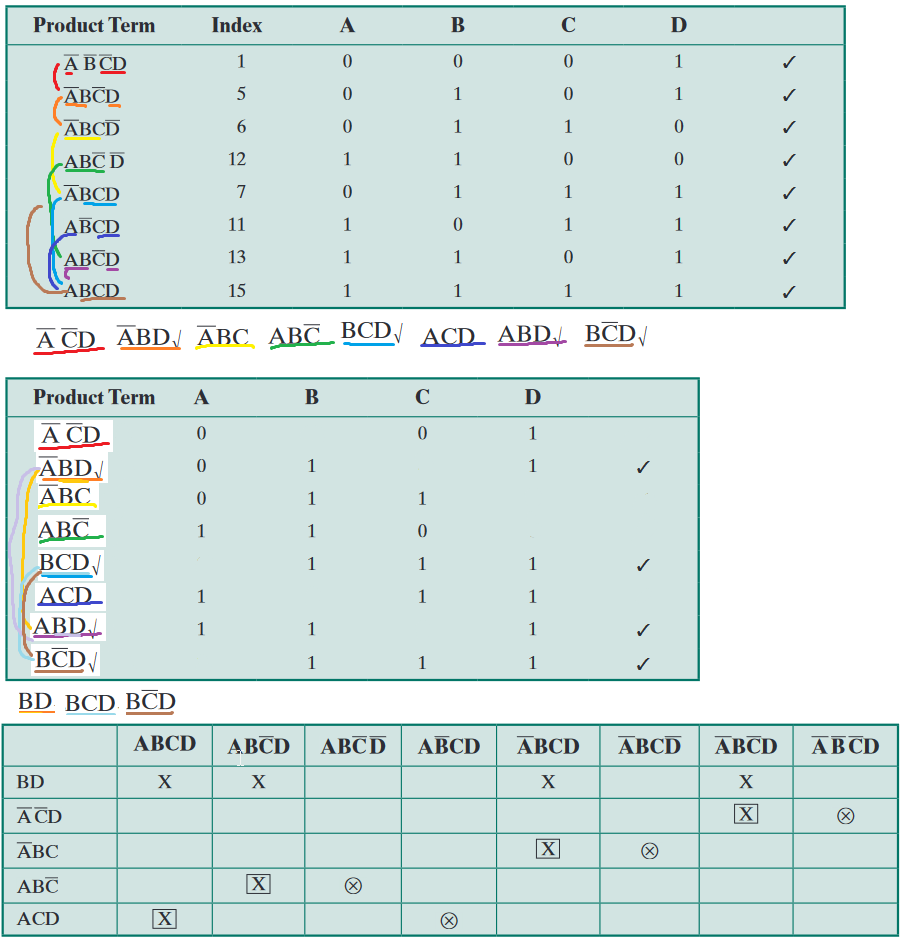
\includegraphics[width=300px]{assets/quine-McCluskey.png}
					\centering
					\caption{Example of the method on \\$F=ABCD+AB\overline{C}D+AB\overline{C}\overline{D}+A\overline{B}CD+\overline{A}BCD+\overline{A}BC\overline{D}+\overline{A}B\overline{C}D+\overline{ABC}D$\\
					Which result in the list $F=AB\overline{C}+ACD+\overline{A}BC+\overline{AC}D$}
				\end{figure}
			\subsection{Circuits}
				\subsubsection{Multiplex}
					Multiplex is a circuit of which a number of inputs label D0,D1,...,DN is wired to an output F.\\
					To controle which input determine the F value, the required number of selection inputs are used called S1,S2...,SN.\\
					So for a 4 input it would require two S inputs.\\
				\subsubsection{Decoders and encoders}
					A decoder is a circuit with a number of output lines, with only one asserted at the time.\\
					In general a decoder has $n$ input and $2^n$ outputs and can be usefull for writting a specific sequence of bits according to a simple code.\\
					An encoder will then be the inverse of the decoder.
				\subsubsection{Read-only Memory}
					As in the name this is memory, which can only be read from and are not programmable.\\
					This is implmented using a decoder and a set of OR gates.\\
					This is done by the a number inputs representing the placement of data and the OR gates each give out the value at the address.
				\subsubsection{Sequential circuits}
					Unlike combinational circuits as above a sequential circuits ouputs are depending on current inputs and the current state.\\
					The most simple form is a flip-flop, which is able to store one bit of data.\\
					There are different types of flip flops with different properties
					\begin{figure}[h!]
						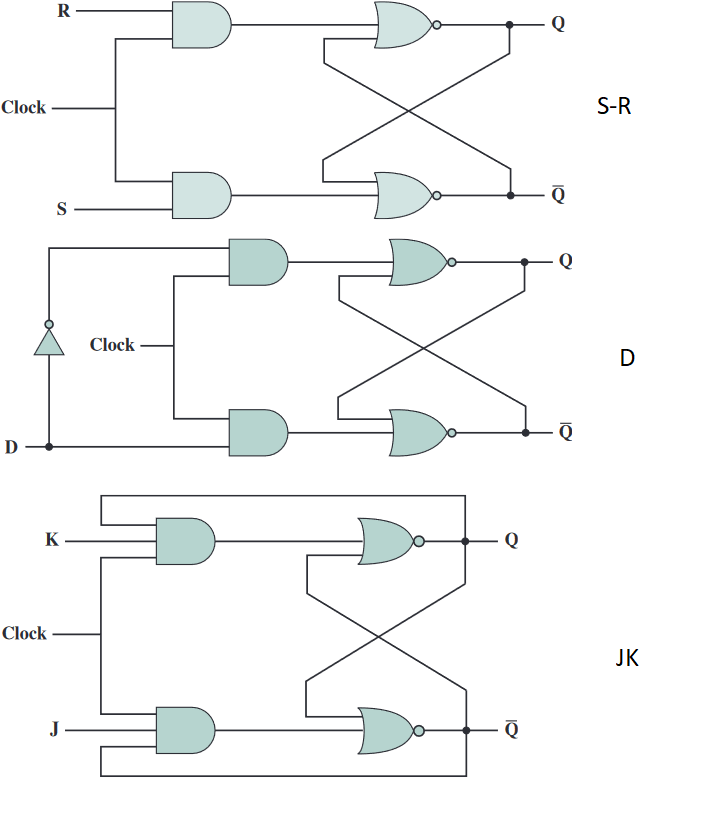
\includegraphics[width=300px]{assets/flipFlops.png}
						\centering
						\caption{Different types of flip flops}
					\end{figure}
					The SR flip flop can not have both S and R be 1 but is the most simple, with a on (S) and off (R)\\
					The D flip flop has a single switch for both on and off\\
					The JK flip flop can have both inputs be 1 and will simply result in Q being 0\\
					These flips flops can then be made in parrallel forming a register, or by as a shift register which has flip flops in series and are sending data down the series at each clock cycle with only input at the front.\\
					Another use case is a series of flip flops which creates a ripple counter or assyncronous counter, which when incrementet the effect ripples through all the other flip flops.\\
					Synchronous counters have the clock going into every flip flop. It can be observed that when counting in binary the first bit, simply flips on every count, the next bits flips when the right bit is 1.\\
					\begin{figure}[h!]
						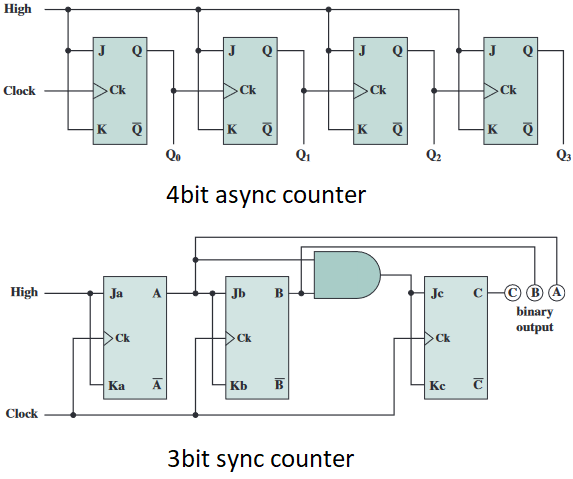
\includegraphics[width=300px]{assets/counters.png}
						\centering
						\caption{Two implmentations of binary counters}
					\end{figure}
				\subsubsection{Programmable logic devices}
					PLD are general-purpose chips.\\
					There are different types of PLD
					\begin{itemize}
						\item PLA - Programmable logic array, is circuit which allows a number of inputs in both normal and negated form, which goes into an array of and gates, which output are wired up to an OR array into the outputs. This takes advantage of SOP binary form
						\item FPGA - Field programmable gate array, is a circuit consisting og a logic block, which are programmable using flip flops, I/O blocks and interconnect which connects the I/O block to the internal logic blocks
					\end{itemize}
	\section{Instruction sets}
		\subsection{Machine instructions}
			A machine instruction consist of the following:
			\begin{itemize}
				\item Operation code - the code which describe the operation to be performed called opcode
				\item Source operand reference - The operation may one or more source reference for the operation
				\item Result operand reference - The reference to the result of the operation if it exist
				\item Next instruction reference - The reference which hold the next instruction for after the execution
			\end{itemize}
			The next instruction reference and result reference can reference memory in different sources:
			\begin{itemize}
				\item Main or virtual memory
				\item Processor register - in some cases one or more registers may contain memory addresses which can be reference by the register name
				\item Immediate - The reference may be contained in the current instruction
				\item I/O device 
			\end{itemize}
			When referencing instruction the opcode is most often represented as abbreviation called mnemonics, such as ADD\\
			Instructions can be of the following types
			\begin{itemize}
				\item Data processing - Artihmetid and logic instructions
				\item Data storage - movement of data from and to registers and memory locations
				\item Data movement - I/O instructions
				\item Control - Test and branch instructions
			\end{itemize}
			Instructions may be designed to use 
			\begin{itemize}
				\item 0 references - This will then use the stack for references
				\item 1 referenece - Performs the instruction on and saves in a common accumulator register or something alike which the instruction is used upon 
				\item 2 references - Performs the instruction and saves it in the first register
				\item 3 references - Performs instruction and first two references and saves in the last reference
			\end{itemize}
			When designing a set of instruction there are multiple questions have to be considered
			\begin{itemize}
				\item Operation repertoire - How many and which operations should be in the set
				\item Data types - Which data types should be avaliable
				\item Instruction format - Instruction lengthm number of addresses, size of varius field and so on
				\item Registers - Number of registers which should be referenceable and what their use should be
				\item Addressing - In which mode an address of an operand is specified
			\end{itemize}
		\subsection{Types of operands}
			For numbers there are 3 different types 
			\begin{itemize}
				\item Binary integer or binary fixed point - The classic integer in binary form
				\item Binary flaoting point - here the first bit mean the sign(1 = negative) the nest 8 bits are the exponent and the next 23 are the mantisse for the 32 bit version
				\item Packed decimal - used to avoid a lot of conversion, such every decimal is represented with 4 bits, and (1101) means - and (1100) means +
			\end{itemize}
			For representing characters 8 binary bits can be used with standards by ASCII, whcih dictates what the different binary combination represent.\\
			The x86 can deal with data types of 8 (byte), 16 (word), 32 (doubleword), 64 (quadword), and 128 (double quadword)\\
			ARM processors support data types of 8 (byte), 16 (halfword), and 32 (word) bits in length.\\
		\subsection{Types of operations}
			A useful and typical categorization is the following: 
			\begin{itemize}
				\item Data transfer - Calculate the memory address based on address mode, if virtual translate to real memory, detemine if data is not cached and issur a command to the memory module.
				\item Arithmetic - Different kind of matematic operations and may include data movement for the operation
				\item Logical - Logical operations such as XOR, right shift, left shift or rotate on binary data
				\item Conversion - Conversion between binary and decimal aswell as operation conversion between 8 bit and such
				\item I/O - Instructions for data movement in and out of the system
				\item System control - Privelege function often reserved to operation system, such as alter register control or modifying storage protection key.
				\item Transfer of control - Operations for changing execution with: branching on condition (if and loops), skip on condition (skip out loop or flow), call a block of code and return to current code (function calling) is done by calling it and pushing parameters and return to stack in a stack frame. 
			\end{itemize}
			When using conditions it refers to one of the architectures flags, which may be raised during instructions.\\
			For x86 the call specificly does
			\begin{itemize}
				\item Push the return point on the stack
				\item Push the current frame pointer on the stack
				\item Copy the stack pointer as the new value of the frame pointer
				\item Adjust the stack pointer to allocate a frame
			\end{itemize}
			This can be done manually by instructions or by the ENTER instruction though it takes 10 cycles instead of 6.\\
			MMX instructions are also exclusive to x86 and are instruction which can operate on multiple smaller data set by combining them into 32 or 64 bit chunks.\\
			This allows the instruction to work in parrallel on things like image processing where pixels are gathered in larger chunks.\\
			
			
			
			
				
\end{document}
